\documentclass{letter}
\usepackage[hmargin=1in,bottom=0.5in]{geometry}
\usepackage{fancyhdr}
\usepackage{graphicx}
\usepackage{fontspec} 
\renewcommand{\headrulewidth}{0pt}
\fancypagestyle{firstpage}{\fancyhf{}\fancyhead[L]{
\includegraphics[height=0.4in, keepaspectratio=true]{bates-wordmark-201.eps}\\Department of\\Physics and Astronomy}\cfoot{44 Campus Ave | Lewiston, ME 04240 | (207) 786-6325}}
\fancypagestyle{plain}{\fancyhf{}\fancyhead[L]{
\includegraphics[height=0.4in, keepaspectratio=true]{bates-wordmark-201.eps}\\Department of\\Physics and Astronomy}\cfoot{44 Campus Ave | Lewiston, ME 04240 | (207) 786-6325}}

\setromanfont[Mapping=tex-text]{Linux Libertine O}

\begin{document}
\begin{letter}{}
  \opening{Dear Editor:}

  We are submitting a manuscript, ``The Magnetorotational Instability Prefers Three Dimensions,'' for consideration in \emph{Nature Physics}.
The magnetorotational instability (MRI) is an extremely important part of astrophysical fluid dynamics, as it is believed to play a key role in accretion disks around compact objects and may also play an important role in stellar interiors.
There are several active laboratory campaigns attempting to make an experimental confirmation of the instability.

Our work demonstrates for the first time that the most unstable MRI mode is three-dimensional at onset when the shear that drives it is close to its critical value.
Previously, based on theoretical and numerical work far from critical shear, the dominant MRI modes were assumed to be axisymmetric.
The conditions for three-dimensional instability are likely to be very common, as driving the flow to near-critical shear is how the instability saturates in systems like stars and laboratory experiments.
This process is similar to convection erasing the background entropy gradient or Taylor-Couette instability forcing the angular momentum gradient toward marginal stability.
%Thus, in the context of stellar interiors and the laboratory experiments seeking to confirm the existence of the MRI, near-critical shear is in fact a very important regime.
The implication of a three-dimensional MRI are twofold: the non-normal nature of the linear operator driving the instability implies that transient growth is always important in the linear phase.
More importantly, the existence of a three-dimensional unstable mode implies that the linear MRI may drive direct dynamo action, amplifying magnetic fields even in the absence of turbulence driven by secondary instabilities.

Our results have important implications for both laboratory studies of the MRI as well as its effects in stellar interiors. 
However, the MRI is also an important magnetohydrodynamic process in its own right.
In particular, it is of interest to plasma physicists as a potential dynamo mechanism.
Our work suggests the existence of a new, laminar dynamo solution.
Such a solution is of fundamental importance in understanding dynamo generated magnetic fields, which are essential to Solar, geo-, and planetary physics.
It also bears deep connections to viscoelastic Taylor-Couette flow that have been studied in the fluid dynamics community. 
Thus, because our work constitutes an important new direction in MRI and dynamo research, we believe it is well suited for the diverse readership of \emph{Nature Physics}. We look forward to corresponding further with you about our work.

\closing{Sincerely, \\
\fromsig{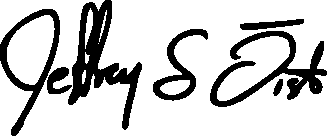
\includegraphics[scale=0.5]{jso_sig.pdf}}\\
\fromname{Jeffrey S. Oishi,\\on behalf of the authors:\\
Geoffrey M.\ Vasil\\
Morgan Baxter\\
Andrew Swan\\
Keaton J. Burns\\
Daniel Lecoanet\\
Benjamin P. Brown}}

\end{letter}
\end{document}


%  LocalWords:  Magnetorotational magnetorotational axisymmetric geo
%  LocalWords:  Couette magnetohydrodynamic viscoelastic Oishi Vasil
%  LocalWords:  Lecoanet
%%% Local Variables: 
%%% coding: utf-8
%%% mode: latex
%%% TeX-engine: xetex
%%% End: 